\documentclass[11pt]{beamer}

%START To get MATLAB environment
\usepackage[numbered,framed]{matlab-prettifier}
%\usepackage{filecontents}

\let\ph\mlplaceholder % shorter macro
\lstMakeShortInline"

\lstset{
	style              = Matlab-editor,
	basicstyle         = \tiny \ttfamily,
	escapechar         = ",
	mlshowsectionrules = true,
}

%\renewcommand{\lstlistingname}{Algorithm}% Listing -> Algorithm
\renewcommand{\lstlistingname}{Code}% Listing -> Code
%FINISH To get MATLAB environment

%\usepackage{standalone}
%\graphicspath{{../}{../}}
%\graphicspath{{../../figures/}}

\setcounter{tocdepth}{1}

\usepackage[english]{babel}

\usepackage{amsmath}
\usepackage{amsfonts}
\usepackage{amssymb}
\usepackage{graphicx}
\usepackage{tikz}
\usetikzlibrary{shapes.geometric, arrows}
\tikzstyle{startstop} = [rectangle, rounded corners, minimum width=1.7cm, minimum height=0.7cm,text centered, draw=black, fill=red!30]
\tikzstyle{io} = [trapezium, trapezium left angle=70, trapezium right angle=110, minimum width=1.7cm, minimum height=0.7cm, text centered, draw=black, fill=blue!30]
\tikzstyle{process} = [rectangle, minimum width=1.7cm, minimum height=0.7cm, text centered, draw=black, fill=orange!30]
\tikzstyle{decision} = [diamond, minimum width=1.7cm, minimum height=0.7cm, text centered, text width=1.7cm, draw=black, fill=green!30]
\tikzstyle{arrow} = [thick,->,>=stealth]



\setbeamercovered{transparent}
%\usepackage{enumitem}
%\setlist[itemize]{leftmargin=*}

%\usepackage{mhchem}
%\usepackage[utf8]{inputenc}
%\usepackage[T1]{fontenc}
%\numberwithin{equation}{section}



\author[Jose Mendoza-Cortes]{Prof. Jose L. Mendoza-Cortes}
\title[Machine Learning]{Machine Learning}
%\subtitle{Spring '18}
\institute[]
{\scriptsize 
	Scientific Computing Department, Dirac Science Building \\
	Materials Science and Engineering, High Performance Materials Institute\\
	Florida State University\\
	\href{mailto:jmendozacortes@fsu.edu}{jmendozacortes@fsu.edu}\\[3mm]
	
	Condensed Matter Theory, National High Magnetic Field Laboratory\\%[3mm]
	Florida State University\\	
	\href{mailto:mendoza@magnet.fsu.edu}{mendoza@magnet.fsu.edu}\\[3mm]	
	
	Chemical and Biomedical Engineering \\
	Florida State University | Florida A\&M University | College of Engineering \\
	\href{mailto:mendoza@eng.famu.fsu.edu}{mendoza@eng.famu.fsu.edu}\\[3mm]
	Web: \href{http://mendoza.eng.fsu.edu/}{http://mendoza.eng.fsu.edu/}\\%[1mm]
}  

\date{}
\subject{Theory and Computations in Materials, Chemistry and Physics}

%\usetheme{Berkeley}
%\logo{\includegraphics[scale=0.213]{figures/fsu_logo.png}}
%\addtobeamertemplate{navigation symbols}{}{%
%    \usebeamerfont{footline}%
%    \usebeamercolor[fg]{footline}%
%    \hspace{1em}%
%    \insertframenumber/\inserttotalframenumber
%}
 
\usetheme{Madrid}
%\usecolortheme{beaver}
%\usecolortheme{orchid}

\newif\ifplacelogo % create a new conditional
\placelogotrue % set it to true
\logo{\ifplacelogo
	\includegraphics[width=0.1\linewidth]{figures/fsu_logo.png}
	\includegraphics[width=0.1\linewidth]{figures/famu_logo.png}
	\includegraphics[width=0.1\linewidth]{figures/maglab_logo.png}
	  \fi} % replace with your own command
	  
\definecolor{mycustom}{RGB}{0,0,102}       %102,38,38 %128,0,0
%\definecolor{mycustom}{RGB}{128,0,0}       %102,38,38 %128,0,0
%
%\setbeamercolor{structure}{bg=white, fg=custom}
%\setbeamercolor{caption}{fg=custom}

\definecolor{custom}{cmyk}{1,0.5,0,0.47}       %102,38,38 %128,0,0

\setbeamercolor{structure}{bg=white, fg=custom}
\setbeamercolor{caption}{fg=custom}

\setbeamertemplate{navigation symbols}{} %To remove the navigation symbols

%\setbeamercolor{frametitle}{fg=custom}
%\setbeamercolor{framesubtitle}{fg=custom}
\setbeamercolor{titlelike}{parent=structure,bg=gray!20!white}

\setlength\abovecaptionskip{-3pt}
\setbeamertemplate{caption}{%
	\insertcaptionname\,\insertcaptionnumber:\,\insertcaption
}



\usepackage{hyperref}
\hypersetup{colorlinks=true,
	linkcolor=mycustom,
	urlcolor=mycustom}

\abovedisplayskip=0pt
\belowdisplayskip=0pt

%%%%%%%%%%%%%%%%%%%%%%%%%%%%%%%%%%%%%%%%%%%
% Requires early loading of  package and commands %%%%%%%%%%%%%%%%
%%%%%%%%%%%%%%%%%%%%%%%%%%%%%%%%%%%%%%%%%%%
%\usepackage{ifthen}					% Helps with conditional statements
\usepackage{censor}					% needed to produce ``fill-in-the-blanks'' documents
\usepackage{stackengine}				% required to adjust ``censor commands''
\usepackage{scalerel}				% required to adjust ``censor commands''


%%%%%%%%%%%%%%%%%%%%%%%%%%%%%%%%%%
% Begin Work On It %%%%%%%%%%%%%%%%%%%%%%%%
%%%%%%%%%%%%%%%%%%%%%%%%%%%%%%%%%%
% It would be great, if this would work
%\usepackage{dashrule}
%\renewcommand\censorrule[1]{\protect\hdashrule[-0.3mm]{#1}{0.1pt}{1pt 5pt}}
%
%This is for the mean time
\renewcommand\censorrule[1]{\protect{\color{gray!35}{\rule[\censorruledepth]{#1}{\censorruleheight}}}}

%%%%%%%%%%%%%%%%%%%%%%%%%%%%%%%%%%
% End Work On it %%%%%%%%%%%%%%%%%%%%%%%%%
%%%%%%%%%%%%%%%%%%%%%%%%%%%%%%%%%%
% Adjust censoring commands
\censorruledepth=-.5ex
\censorruleheight=.1ex
%%%%%%%%%%%%%%%%%%%%%%%%%%%%%%%
% Color code text in presentation %%%%%%%%%%%%%%
% To easily identify missing text in fill-in-the-blank document 
%%%%%%%%%%%%%%%%%%%%%%%%%%%%%%%
\makeatletter
%%%%%%%

\renewcommand\StopCensoring{%
	\def\censor##1{\textcolor{blue}{##1}}%
	\def\censorX##1{{##1}}% To make the \censorX like it is not existing
	\def\censorbox##1{\bgroup\color{blue}\un@censorbox{##1}\egroup}%
	\let\xblackout\blackout%
}
%%%%%%%
\renewcommand\censor@box[2][]{\fboxsep=0pt\fbox{\color{white}%
		#1\setbox0\hbox{#2}%
		%                      \rule[-\the\dp0]{\the\wd0}{\the\ht0+\the\dp0}}
		\rule[-\the\dp0]{\the\wd0}{\the\ht0+\the\dp0}}
}
%%%%%%%%
%\newcommand\m@cenword[1]{\ThisStyle{%
%\stackengine{\mcensorruledepth}{$\SavedStyle\phantom{#1}$}%
%{\rule{\widthof{$\SavedStyle#1$}}{\the\censorruleheight}}{U}{c}{F}{T}{L}}
%}
\newcommand\m@cenword[1]{\ThisStyle{% 
		\textcolor{gray!35}{\stackengine{\mcensorruledepth}{$\SavedStyle\phantom{#1}$}% 
			{\rule{\widthof{$\SavedStyle#1$}}{\the\censorruleheight}}{U}{c}{F}{T}{L}}
	}}
	%%%%%%%
	\newcommand\mblackout[2][\dp\strutbox]{%
		\let\@cenword\m@cenword%
		\def\mcensorruledepth{#1}%
		\blackout{{#2}}%
		\let\@cenword\sv@cenword%
	}
	%%%%%%%
	% Switch between ``all'' censored and ``half'' censored commands 
	%\let\censorX\censor
	%%%%%%%
	\StopCensoring	
	\makeatother
	%%%%%%%%%%%%%%%%%%%%%%%%%%%%%%%%%%%%%%%%%%%%%%
	%% Begin Censor Adjustments %%%%%%%%%%%%%%%%%%%%%%%%%%%%%%
	%%%%%%%%%%%%%%%%%%%%%%%%%%%%%%%%%%%%%%%%%%%%%%
	% Use these commands to manually switch  ``fill-in the blank'' on and off
	%\renewcommand\StopCensoring{%
	%	\def\censor##1{\textcolor{green}{##1}}%
	%	\def\censorX##1{{##1}}% To make the \censorX like it is not existing
	%	\def\censorbox##1{\bgroup\color{blue}\un@censorbox{##1}\egroup}%
	%	\let\xblackout\blackout%
	%}
	%%%%%%%%%%%%
	%%%%%%%%%%%
	\RestartCensoring
	\StopCensoring
	%%%%%%%%%%%%%%%%%%%%%%%%%%%%%%%%%%%%%%%%%%%%%%
	%% End Censor Adjustments %%%%%%%%%%%%%%%%%%%%%%%%%%%%%%%
	%%%%%%%%%%%%%%%%%%%%%%%%%%%%%%%%%%%%%%%%%%%%%%
	\usepackage{pgfpages}
		\pgfpagesuselayout{2 on 1}[letterpaper,%landscape,
		border shrink=5mm]
	



\begin{document}
\placelogofalse
%\placelogotrue % turn the logo off \usetheme{Madrid}
\maketitle

%\placelogofalse % turn the logo off

\section{Notes}

%*****************

%*****************

\begin{frame}
	\frametitle{Overview}
	%\centering
	
	\begin{block}{}
		\centering
		Lecture: MATLAB Programming Environment \\
		Lecture: Vector and Matrix Operations
	\end{block}
	
	\begin{minipage}[t]{0.45\linewidth}
		\begin{enumerate}
			\item MATLAB Environment 
			%\item Concatenation 
			%\item Loops
			%\item Ifs
		\end{enumerate}
	\end{minipage}
	%\onslide<2->
	\begin{minipage}[t]{0.45\linewidth}
		\vspace{11pt}
		\textit{``The first principle is that you must not fool yourself - and you are the easiest person to fool''}\\
		\vspace{25pt}
		-Richard P. Feynman
		\vfill
	\end{minipage}
	
\end{frame}




\section{Notes}
%*****************
\begin{frame}
	\frametitle{\secname: Programming}
	%	\begin{figure}[h!]
	%		\centering
	%		\includegraphics[height=0.86\textheight]{figures/flowchart}
	%	\end{figure}
	
	\begin{minipage}[t]{\linewidth}
		\vspace{-13pt} \centering
		\textbf{A computer does two things, and two things only: it performs calculations and it remembers the results of those calculations}
	\end{minipage}
	\begin{minipage}[t]{\linewidth}
		\vspace{-3pt}
		\begin{figure}[h!]
			\centering
			\includegraphics[height=0.8\textheight]{figures/flowchart}
		\end{figure}
	\end{minipage}	
	
\end{frame}


%*****************
\begin{frame}
	\frametitle{\secname: Programming}
	\centering
	\begin{minipage}[t]{0.55\linewidth}
		\vspace{-17pt}
		\begin{figure}[h!]
			\centering
			\includegraphics[height=0.85\textheight]{figures/flow1}
		\end{figure}
	\end{minipage}
	\begin{minipage}[t]{0.35\linewidth}
		%	\onslide<2->
		\textbf{Cooking}\\
		\begin{enumerate}
			\setlength{\itemsep}{0pt}
			\item[1.-] Boil water
			\item[2.-] Add water to instant noodle cup
			\item[3.-] Let it be for 3 minutes
			\item[4.-] Taste it and see if you like it
			\item[5.-] Add some sauce or other things
			\item[6.-] stir
			\item[7.-] EAT
		\end{enumerate}
	\end{minipage}	
\end{frame}


%*****************
\begin{frame}[fragile=singleslide]
	
	\frametitle{\secname: MATLAB}
	\centering
	\begin{minipage}[t]{0.5\linewidth}
		\vspace{-15pt}
		\begin{figure}[h!]
			\centering
			\includegraphics[height=0.45\textheight]{figures/1matlab}
		\end{figure}
		\vspace{-7pt}
		\textbf{Why MATLAB is great?}
		\begin{itemize}
			\setlength{\itemsep}{0pt}
			\item[*] It was built with the intention to work with \censor{matrices} (e.g. like column vectors)
			\item[*] MATLAB is at least as good as your calculator
		\end{itemize}
	\end{minipage}
	\begin{minipage}[t]{0.45\linewidth}
		\vspace{-15pt}
		\begin{verbatim}
		a = 2;
		b = 3;
		a + b
		v=[0 1 2]
		u=[3; 4; 5]
		w=[1 2 3; 4 5 6; 7 8 9]
		transpose(u)
		z = u'
		v + u'
		u(2)		
		v(1)
		w(:,2)
		w(2,:)
		x=[5 6 7]
		x * v % invalid, why?
		x .* v % valid. why? 
		% This is IMPORTANT!
		\end{verbatim}
	\end{minipage}
	
\end{frame}


\section{Notes}
%*****************
\begin{frame}[fragile]
	
	\frametitle{\secname: MATLAB- Concatenation (\href{http://www.mathworks.com/help/matlab/math/creating-and-concatenating-matrices.html}{More info})}
	\centering
	\begin{minipage}[t]{0.45\linewidth}
		\vspace{-15pt}	
		\begin{verbatim}
		C=1:0.5:2.5
		C=[1:0.5:2.5]
		C(2)    => 1.5
		C(1,2)  => 1.5
		C2=C'
		C2(2)   => 1.5
		C2(2,1) => 1.5	
		
		%Concatenation
		c=1:3   => [1 2 3]
		d=2:3   => [2 3]
		e=[c d] => [1 2 3 2 3]
		d2=3:4  => [3 4]
		c2=2:4  => [2 3 4]
		
		d3=[d;d2] => 2by2 matrix
		c3=[c c2] => 2by3 matrix		
		\end{verbatim}
	\end{minipage}
	\begin{minipage}[t]{0.5\linewidth}
		\vspace{-15pt}
		%\onslide<2->
		\textbf{Semicolon operator;}\\
		When used at the end of the line, it \censor{suppress} any display of numerical operations.
		When used in brackets, it does a \censor{vertical} concatenation.
		\vspace{-7pt} 
		\begin{verbatim}
		s=[d;c] % Error, columns match?
		f=[c;c3] % Error, rows match?
		\end{verbatim}
		Same Height
		\vspace{-7pt}
		\begin{center}
			\includegraphics[width=0.95\linewidth]{figures/ch_data_struct1}\
		\end{center}
		\vspace{-7pt}	
		Not the Same Height
		\vspace{-7pt}	
		\begin{center}
			\includegraphics[width=0.95\linewidth]{figures/ch_data_struct2}\
		\end{center}
		
	\end{minipage}
	
\end{frame}



%*****************
\begin{frame}[fragile]
	
	\frametitle{\secname: MATLAB - Loops 
		(\href{http://www.mathworks.com/help/matlab/matlab_prog/loop-control-statements.html}{More info})}
	%\centering
	%\begin{center}
	%	\textbf{There are two types of loops in MATLAB:}
	%\end{center}
	
	\begin{block}{}
		\centering There are two types of loops in MATLAB:
	\end{block}
	
	\begin{minipage}[t]{0.55\linewidth}
		1. \verb|for| statements loop a specific number of times, and keep track of each iteration with an \censor{incrementing} index variable.
		\begin{verbatim}
		for i=1:10
		i
		end
		\end{verbatim}
	\end{minipage}
	\hspace{5pt}
	\begin{minipage}[t]{0.4\linewidth}
		2. \verb|while| statements loop as long as a condition remains \censor {true}.
		\begin{verbatim}
		i=1
		while i < 10
		i=i+1
		end
		\end{verbatim}	
	\end{minipage}
	
	\vspace{15pt}
	Either can be used for this purpose. Another way to look at them is:
	\begin{itemize}
		\item \verb|for| loops continue a set number of iterations
		\item \verb|while| loops continue until a condition is met
	\end{itemize}
	
	%\onslide<2->
	\begin{exampleblock}{Class Exercise}
		Draw the flow diagram of each case
	\end{exampleblock}
	
\end{frame}



%*****************
\begin{frame}[fragile]
	
	\frametitle{\secname: MATLAB - Loops 
		(\href{http://www.mathworks.com/help/matlab/matlab_prog/loop-control-statements.html}{More info})}
	%\centering
	\vspace{-3pt}
	\begin{minipage}[t]{0.47\linewidth}
		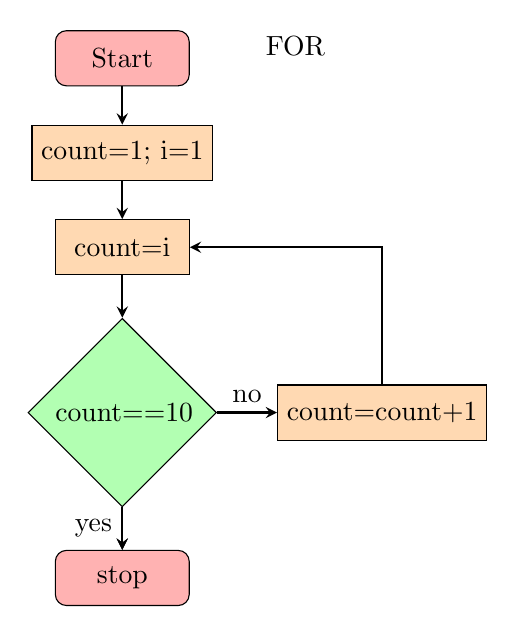
\begin{tikzpicture}[node distance=1.2cm]
		\node (start) [startstop] {Start};
		\node (pro1) [process,  below of=start] {count=1; i=1};
		\node (pro2) [process,  below of=pro1] {count=i};
		\node (dec1) [decision, below of=pro2, yshift=-0.9cm] {count==10};
		\node (pro2a) [process, right of=dec1, xshift=2.1cm] {count=count+1};
		\node (stop) [startstop,  below of=dec1, yshift=-0.9cm] {stop};
		\draw [arrow] (start) -- (pro1);
		\draw [arrow] (pro1) -- (pro2);
		\draw [arrow] (pro2) -- (dec1);
		\draw [arrow] (dec1) -- (stop);
		\draw [arrow] (dec1) -- node[anchor=south] {no} (pro2a);
		\draw [arrow] (dec1) -- node[anchor=east] {yes} (stop);
		\draw [arrow] (pro2a) |-node[anchor=south, xshift=-1.1cm, yshift=2.3cm] {FOR} (pro2);
		\end{tikzpicture}
	\end{minipage}
	\hspace{9pt}
	\begin{minipage}[t]{0.47\linewidth}
		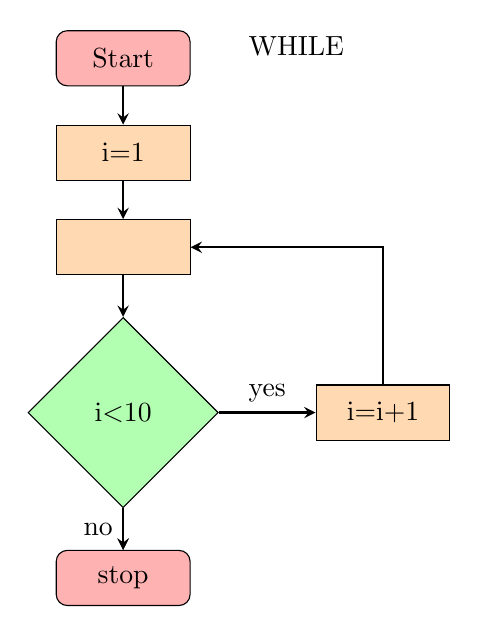
\begin{tikzpicture}[node distance=1.2cm]
		\node (start) [startstop] {Start};
		\node (pro1) [process,  below of=start] {i=1};
		\node (pro2) [process,  below of=pro1] {};
		\node (dec1) [decision, below of=pro2, yshift=-0.9cm] {i$<$10};
		\node (pro2a) [process, right of=dec1, xshift=2.1cm] {i=i+1};
		\node (stop) [startstop,  below of=dec1, yshift=-0.9cm] {stop};
		\draw [arrow] (start) -- (pro1);
		\draw [arrow] (pro1) -- (pro2);
		\draw [arrow] (pro2) -- (dec1);
		\draw [arrow] (dec1) -- (stop);
		\draw [arrow] (dec1) -- node[anchor=south] {yes} (pro2a);
		\draw [arrow] (dec1) -- node[anchor=east] {no} (stop);
		\draw [arrow] (pro2a) |-node[anchor=south, xshift=-1.1cm, yshift=2.3cm] {WHILE} (pro2);
		\end{tikzpicture}	
	\end{minipage}
	\vspace{-1mm}
		\begin{exampleblock}{}
			\footnotesize In class we discuss how to make a \verb|while| loop infinetly, do you remember how?
		\end{exampleblock}	
\end{frame}

%*****************
\begin{frame}[fragile]
	
	\frametitle{\secname: MATLAB - Loops 
		(\href{http://www.mathworks.com/help/matlab/matlab_prog/loop-control-statements.html}{More info})}
	%\centering
	\begin{block}{}
		More on Loops and Conditions
	\end{block}
	
	\begin{minipage}[t]{0.55\linewidth}
		%\vspace{-5pt}	
		\begin{verbatim}
		for i=1:5 % try for i=1:2:10
		x(i)=i
		v(i)=i^2
		end
		plot(x,v)
		\end{verbatim}
		As some of you might have recognized, you can get the same effect by the following:
		\begin{verbatim}
		x=[1:1:5];
		v=x.^2; % notice our friend
		".^", what if you used only ^?
		plot(x,v)
		\end{verbatim}
	\end{minipage}\hspace{7pt}
	\begin{minipage}[t]{0.42\linewidth}
		%\vspace{-15pt}
		\textbf{Example}\\
		\begin{center}
			Solve $\sum_{i=1}^{10}i^2$
		\end{center}
		
		\begin{block}{}
		\textit{Remember it is a good technique to start with your flow diagram}
		\end{block}
		
		%\onslide<2->
		\begin{verbatim}
		sum = 0
		for i=1:10
		sum=sum+i^2
		end	
		\end{verbatim}
		
		
	\end{minipage}
	
	
\end{frame}


%*****************
\begin{frame}[fragile]
	
	\frametitle{Lecture: MATLAB - Decisions if/elseif/else
		(\href{http://www.mathworks.com/help/matlab/ref/if.html}{More info})}
	%\centering
	\vspace{-5pt}	
	\begin{minipage}[t]{0.47\linewidth}
		%\vspace{-15pt}	
		\textbf{Example:}
		\begin{verbatim}
		% note the == to test 
		% equality
		
		if i==1 
		disp('i=1')
		elseif i<1
		disp('i<1')
		else
		disp('i>1')
		end
		
		%Now give different values 
		%to i and test it
		\end{verbatim}
	\end{minipage}
	\begin{minipage}[t]{0.47\linewidth}
		%\onslide<2->
		\textbf{Problem:}
		A single iteration can be skipped by using the "continue" command
		
		Solve $\sum_{i=1}^{10}i^2$ with $i\neq 4$\\
		is equivalent to $\sum_{i=1}^{3}i^2+\sum_{i=5}^{10}i^2$
		%\vspace{-5pt}
		\begin{verbatim}
		sum=0
		for i=1:10
		if i=4
		continue
		end
		i   
		sum = sum + i^2
		end
		%What happen if you comment out
		%the continue subroutine
		\end{verbatim}	
		\vspace{-5mm}
	\end{minipage}
	
		\begin{exampleblock}{}
			There are other ways to solve this problem. Can you write them down?
		\end{exampleblock}	
	
\end{frame}




%*****************

\begin{frame}[fragile]
	\frametitle{Review}
	%\centering
	
	\begin{block}{}
		\centering
		Notes: MATLAB Programming Environment \\
		Notes:Vector and Matrix Operations
	\end{block}
	\begin{minipage}[t]{0.43\linewidth}
		\vspace{-10pt}
		\begin{enumerate}
			\item Programming Environment
			\item Vectors 
			\item Matrix Operations
		\end{enumerate}
		\vspace{-10pt}
		\begin{alertblock}{Remember}
			\begin{itemize}
				\item The percent sign \verb|%| denotes
				the start of a \censor {comment}, and MATLAB ignores it.\\
				\item The operators \verb|.*| tellw MATLAB to do element by element \censor{multiplication}. The sign ./ tells an element by element \censor {division}. 
			\end{itemize}
		\end{alertblock}
	\end{minipage}
	\hspace{10pt}
	\begin{minipage}[t]{0.51\linewidth}
		\vspace{-15pt}
		\begin{block}{How to look for Help}
			\begin{itemize}
				\item You can always get help on a command (say \verb|plot|) by typing \verb|help plot| in MATLAB's command window.
				\item You can also use the upper right corner section called ``Search Documentation''
				\item And of course, there is also \href{www.google.com}{Google}. Just make sure that in your search you include 'MATLAB and the question'
			\end{itemize}			
		\end{block}
	\end{minipage}
	
\end{frame}

%*****************

%\placelogotrue

%\begin{frame}
%	\frametitle{See you next class}
%	\vspace{-25pt}
%	
%	\textit{``Just as there is not royal road to geometry, there is no royal road to programming''}.- Euclid and J. V. Guttag
%	\vspace{7pt}
%	
%	\textit{The computer will do what you TELL them to do NOT what you WANT them to do}.- Someone in the Internet (Perhaps)
%	\vspace{7pt}	
%	
%	\textit{Think twice, code once}.- Anonymous
%	\vspace{7pt}
%	
%	\textit{The sooner you start to code, the longer the program will take}.- R. Carlson\vspace{7pt}
%	
%	\textit{Any fool can write code that a computer can understand. Good programmers write code that humans can understand}.- M. Fowler
%	\vspace{7pt}
%	
%	\textit{Simplicity is the soul of efficiency}.- A. Freeman
%	\vspace{7pt}
%	
%	\textit{If you cannot grok the overall structure of a program while taking a shower, you are not ready to code it}.- R. Pattis
%	
%\end{frame}

\section{Appendix: Scripts included}

%\subsection{}

\begin{frame}
\frametitle{\secname}

\vspace{-7pt}
\lstinputlisting[caption={Introduction.m}]{N1_Notes_on_programming_Introduction/Introduction.m}

\vspace{-7pt}
\begin{exampleblock}{}
	Try these commands in your own workstation, i.e. have the lectures on one half side of your screen and Matlab/Octave-GUI on the other half. %This is the best approach to learning this.   
\end{exampleblock}

\vspace{-3pt}
\begin{alertblock}{}
	Check the scripts/functions under the directory for this note number (X): \newline
	/NX\_Notes\_directory
\end{alertblock}

\end{frame}	

%\placelogofalse


\end{document}